\documentclass{SCreport}
\usepackage[utf8]{inputenc}
\usepackage[T1]{fontenc}
\usepackage{caption}
\usepackage{float}
\captionsetup{font=small}
\setcounter{tocdepth}{2}
\newcommand\github
{https://github.com/PacificCommunity/ofp-sam-transition-plan/blob/main}
\newcommand\h[1]{\hspace{#1}}
\newcommand\present{\github/presentations}
\newcommand\I[1]{\rule{0pt}{#1}}
\reporttype{SC21}
\reportauthor{A.~Magnusson\footnote{\spc}, N.~Davies\footnote{TeTakina Ltd},
  G.~Pilling$^1$, P.~Hamer$^1$}
\reporttitle{Scoping the Next Generation of Tuna Stock Assessment
  Software:\\Progress Report and Outline of Options (Project 123)}
\reportnumber{\tpnum/SA-WP-01}
\reportdate{17 July 2025}
\setlength\tolerance{2000}
\hyphenation{decisions future supported assessments acknowledged marlin software
  assessment replacement consideration development traditional collaboration
  benefits exercises embarking modules variety structure denmark university
  valuable inter-national input}
\begin{document}

\wcpfctitlepage

\tableofcontents
\newpage

\section{Executive summary}

The 3-year Project 123 aims to evaluate features and capabilities that will be
important in future tuna assessments, explore fitting models to tuna data using
existing software platforms, guide decisions on the type of new software
development required, and establish collaboration with tuna Regional Fisheries
Management Organizations (RFMOs) and research labs to achieve these goals.

At SC20, ISG-09 reviewed the scoping of next-generation tuna stock assessment
software and supported prioritizing practical tasks, including transitioning
swordfish and striped marlin assessments to Stock Synthesis and testing
simplified models for yellowfin tuna. Members acknowledged the need to focus on
immediate assessment priorities while keeping longer-term software development
under consideration, depending on available resources and capacity. (SC20
Summary Report, Attachment E).

SC21 will review the progress of Project 123, which explores the transition to
next-generation stock assessment software for tuna fisheries. The project report
i) evaluates the benefits, limitations, uncertainties, and resource implications
associated with each software platform under consideration; ii) evaluates the
feasibility of analyzing tagging data independently from the main stock
assessment models, a potential strategy to reduce model complexity while
maintaining scientific robustness; and iii) identifies key analytical features
and technical capabilities that future stock assessment platforms should
incorporate, such as support for spatial structure, tagging integration, and
flexibility for multi-species and multi-fleet assessments, to ensure that WCPFC
assessments remain scientifically credible, transparent, and adaptable to
evolving fishery and management needs.

SC21 will provide feedback on the progress of the project as needed.

\vspace{4ex}

We invite SC21 to:

\begin{itemize}
  \item note that over the next 5+ years, MULTIFAN-CL will begin to be phased
  out as a software platform for WCPFC tuna and billfish stock assessments;
  \item note that in 2025, the two billfish stock assessments, swordfish and
  striped marlin, transitioned from MULTIFAN-CL to Stock Synthesis; and
  \item review and comment on two suggested software development work streams,
  described in this report, providing feedback that will guide the preparation
  of project proposals to be presented to SC22.
\end{itemize}

\section{Introduction}

\subsection{The need to migrate to new software}

Following the retirement of the lead developer of MULTIFAN-CL (MFCL), Dave
Fournier, future advances to the MFCL software are not expected to be as
mathematically innovative as they were in the past. While this does not render
MFCL obsolete in the medium-term, it flags the need to plan and identify whether
alternative existing software exists, or new software must be developed in the
longer-term, to continue to support the specificities and future requirements of
WCPFC tuna stock assessments.

While MFCL (Fournier et al. 1998) continues to be improved to service the WCPFC
tuna assessment needs over at least the next 5+ years, it is important to start
on a phased approach to its replacement. An initial scoping phase is required to
assess what features and capabilities will be important in future assessment
software for tunas. This scoping phase will benefit from input from stock
assessment scientists across global tuna RFMOs. Once this scoping phase is
conducted, consideration of available software packages in relation to the
desired features and capabilities can be conducted. This may identify suitable
existing software that has potential to provide the desired features and/or has
potential to be developed further. Alternatively, it may indicate whether
embarking on development of a new software package is recommended.

There has also been discussion around the need to explore, through
modeling/simulation exercises, the benefits of applying alternative assessment
structures (i.e., length-age structured versus the traditional length-based
age-structured approach of MFCL and Stock Synthesis) before embarking on major
software developments or changing methodology. Similar can be said about
exploring benefits of state-space models and their use of random variables.
Simulation exercises to explore the benefits or drawbacks of alternative model
structures or approaches will also require collaboration across tuna RFMOs and
practitioners experienced in using the alternative approaches and/or software.

An important outcome of this work would be to ultimately have a software package
that has the desired functionality for tuna assessments, not only for WCPFC but
also for other tuna RFMOs, thus creating a user community and ongoing
development support capacity, so as to avoid the current situation we are facing
with MFCL. Wider collaboration in this venture is essential to achieving this
and is expected to be encouraged through this project.

\newpage

\subsection{Project outline}
\label{sec:project-outline}

This initial scoping project is scheduled from 1 Feb 2024 to 31 Dec 2026. It
will:

\begin{itemize}
  \item Evaluate features and capabilities that will be important in future
  tuna assessments\\[-4.5ex]
  \item Explore fitting models to tuna data using existing software
  platforms\\[-4.5ex]
  \item Guide decisions on what kind of new software development will be
  required\\[-4.5ex]
  \item Establish collaboration with tRFMOs and research labs to achieve these
  goals
\end{itemize}

Additional projects can be launched in parallel to develop and test new
software.

It is recommended that from 2027 onwards, the scoping project becomes a
coordination project, until all stocks have transitioned from MULTIFAN-CL and
Stock Synthesis to new software platforms.

The project is divided into stages, as follows:

Year 2024

\begin{enumerate}
  \item Review and identify important features for tuna assessments.\\[-4.5ex]
  \item Identify existing software platforms that have these features or can be
  extended.\\[-4.5ex]
  \item Reach out to and initiate collaboration with model developers.
\end{enumerate}

Years 2025--2026 (subject to SC advice and funding approvals by WCPFC)

\begin{enumerate}\setcounter{enumi}{3}
  \item Explore and compare existing platforms, fitting to SPC tuna
  data.\\[-4.5ex]
  \item Determine which platforms can be considered viable candidates.\\[-4.5ex]
  \item If viable candidate platforms have been identified, plan
  transition.\\[-4.5ex]
  \item If any stocks do not have a viable candidate platform for future
  assessments:\\
  $\Rightarrow$ Launch software development projects to extend platforms or
  create new ones.
\end{enumerate}

Years 2027--2029 (anticipating that the scoping project becomes a coordination
project)

\begin{enumerate}\setcounter{enumi}{7}
  \item Coordinate projects developing new software for tuna
  assessments.\\[-4.5ex]
  \item Coordinate tests and model explorations, applying existing and new
  software\\ platforms to SPC datasets.\\[-4.5ex]
  \item Support transition of MULTIFAN-CL and Stock Synthesis tuna and
  billfish\\
  stock assessments to new software platforms.
\end{enumerate}

See also the project terms of reference in \autoref{sec:tor}.

\section{General plan}

\subsection{Requirements for future assessment software}

\subsubsection{CAPAM 2019}

The CAPAM 2019 Workshop on Next Generation Assessment Models provided an
overview and discussion of existing software, as well as recommendations for
further software development. The review paper resulting from this CAPAM
workshop (Punt et al. 2020) identified a number of model features considered
important in future stock assessment software. The abstract of the review paper
lists these features:

\begin{itemize}
  \item Ability to to capture age and size dynamics simultaneously yet
  computationally efficiently, while also offering the option to run a model as
  purely age-structured for a simple and fast model
  \item Scale from data-rich to data-poor
  \item Include some multispecies capability
  \item More appropriately deal with temporal variation, e.g., random effects
  and state-space models
  \item Better handling of tagging data, e.g., release-conditioned or
  recapture-conditioned model
  \item Ability to use close-kin mark-recapture data
  \item Efficient methods to share parameter priors among stocks, borrowing
  information from similar stocks where more data have been collected
  \item Training programs and documentation
  \item Data entry system that is well documented
  \item Does not require specification of inputs that will not be used in an
  application
  \item Expert system to configure default settings based on best practices
  \item Automatic production of diagnostic statistics
\end{itemize}

The summary table in Punt et al. (2020) adds the following features:

\begin{itemize}
  \item Spatial structure
  \item Multiple fisheries and surveys
  \item Flexible parametrization of the initial conditions
  \item Multiple time steps within a year
  \item Flexible parametrization of growth
  \item Flexible parametrization of natural mortality
  \item Flexible parametrization of fecundity
  \item Flexible parametrization of movement
  \item Multiple recruitment functional forms, including nonparametric
  \item Selectivity as a function of age, size, or both
  \item Multiple selectivity functional forms, including dome-shaped and
  asymptotic
  \item Incorporation of ageing error
  \item Ability to simulate datasets for management strategy evaluation
  \item Prefer statistically based likelihood weighting over subjective choices
  \item Ability to evaluate uncertainty using a variety of statistical methods
  \item Allow time-varying processes, both in biology and fishing processes
\end{itemize}

Further in the text, Punt et al. (2020) add the following features:

\begin{itemize}
  \item Allow for density-dependence at the spatial area level, as well as at
  the stock level
  \item Allow for nesting of spatial scales such that a population model can
  appropriately utilize data types collected at fine scale and coarse spatial
  resolutions
  \item Allow for multiple movement types including advection, diffusion, and
  that movement responds to environmental drivers
  \item Account for multiple hypotheses regarding movement, including age- and
  sex-specific processes processes, as well as density-dependent and
  time-varying movement
\end{itemize}

\subsubsection{International Expert Meeting 2024}

At the launch of this scoping project in 2024, an international expert meeting
was held in two sessions. As a background for the meeting discussion, the
conveners (Magnusson and Davies 2024) highlighted model features that can be
especially relevant in tuna assessments:

\textit{Incorporating data}

\begin{itemize}
  \item Fit to length comps
  \item Fit to weight comps
  \item Fit to tagging data
  \item Fit to CKMR data
  \item Estimate growth curve using otolith data
  \item Utilize tag-recapture growth increment to estimate growth
\end{itemize}

\textit{Specifics}

\begin{itemize}
  \item Age-specific M
  \item Length-specific selectivity
  \item Sex-specific growth and M
  \item Region-specific growth
\end{itemize}

\textit{Dimensions}

\begin{itemize}
  \item Explicit regions with movement
  \item Tracking age and length in population
  \item Time steps within a year
\end{itemize}

\textit{Ecology}

\begin{itemize}
  \item Multispecies interactions
  \item Climate change
\end{itemize}

\textit{Implementation}

\begin{itemize}
  \item Random effects, state space
  \item Parallel computing
  \item Computation time
\end{itemize}

\subsubsection{Conclusion}

\subsection{Possible outcomes and options}

\subsection{SPC plan for transitioning to new software}

\begin{figure}[H]
  \centering
  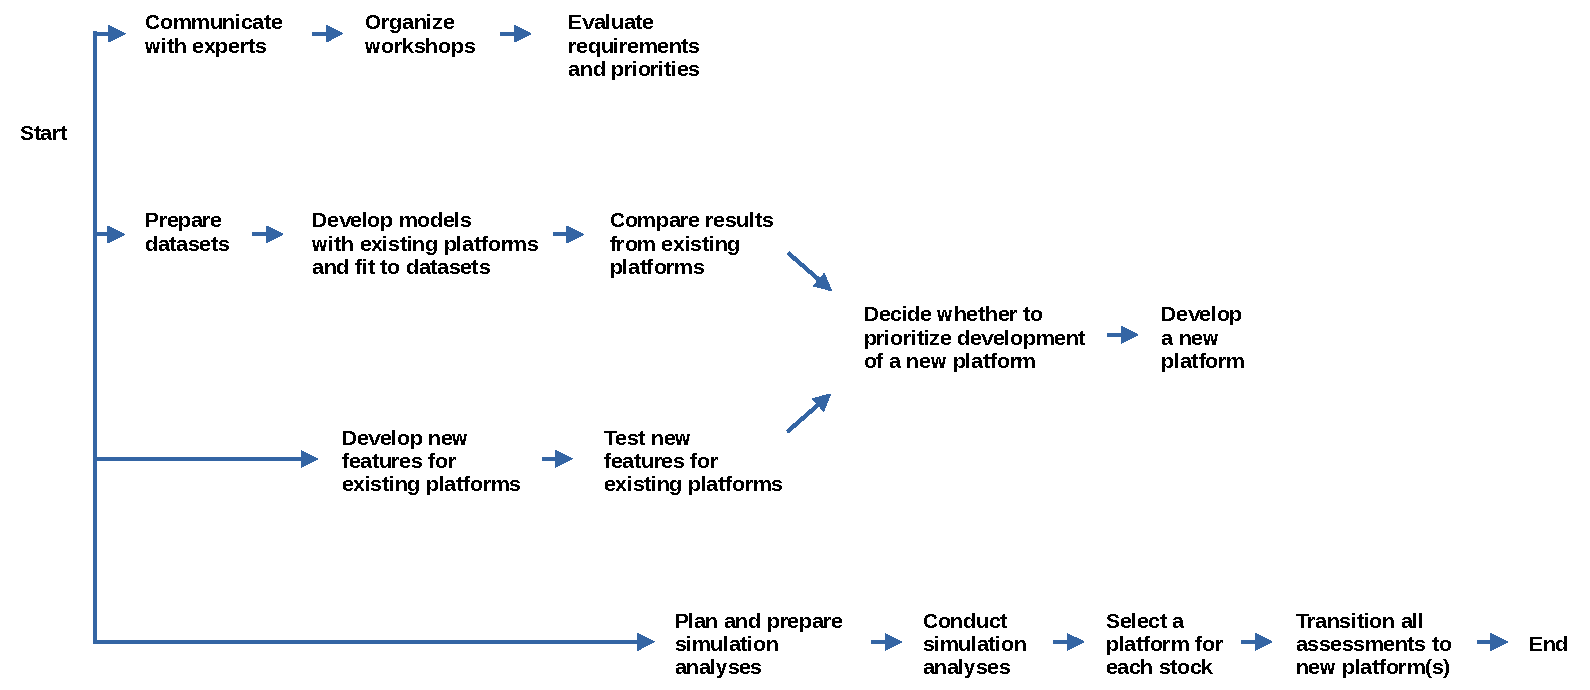
\includegraphics[width=\textwidth]{tasks_no_margin}
  \caption{Overview of steps related to the next generation of tuna stock
    assessment software. Project~123 will focus on the first line of scoping
    tasks (communicate, organize, evaluate) and prepare the ground for
    subsequent lines of tasks (the main project), which will require additional
    funding and resources.}\label{fig:diagram}
\end{figure}

\section{Evaluation of existing software}

\subsection{Stock Synthesis}

Stock Synthesis 3 is used in tuna assessments by the IATTC, IOTC, and ICCAT.
Migrating SPC assessments to Stock Synthesis would lose some of the features
provided by MFCL and this would be transitioning to another platform that is
expected to be phased out in the not-too-distant future. On the other hand,
increasing the use of Stock Synthesis at SPC would facilitate collaboration
between the tRFMOs, including development of future models. It would also
shorten the training time for new SPC stock assessors and make their skills and
experience more transferable to subsequent workplaces. Stock Synthesis
assessments would allow closer comparisons of assessments conducted across RFMOs
and also SPC and the ISC. Stock Synthesis has a large user community that is
relevant for peer reviews and discussing technical decisions. It also comes with
an exceptionally complete suite of tools useful for diagnostics, as well as
automated plots and tables for assessment reports. A possible avenue of
collaborative development is to explore the possibility of enhancing the tag
module, see \autoref{sec:software-early-development}.

\subsection{Gadget}

Gadget 3 is the latest version of Gadget stock assessment platform, implemented
in TMB. It is an age-length structured platform and porting the software to TMB
has resulted in a significant performance gain in terms of computational time.
Gadget has a wide range of features relevant for tuna assessments and a possible
avenue of collaborative development is to test the use of Gadget for a tuna
assessment.

\subsection{sbt}

Used in the assessment of southern bluefin tuna by CCSBT. This package,
implemented in RTMB, stands out as the primary stock assessment software that is
built around close-kin mark-recapture (CKMR) which is a new and important data
type in upcoming SPC tuna assessments. The \textsf{sbt} R package is designed
for a single-region assessment and would require some additional development to
be used for a multiregion assessment. A possible avenue of collaborative
development is to explore the possibility of adding multiregion functionality to
the software.

\subsection{Other}

\begin{itemize}
  \item Casal 2 is the latest version of the Casal stock assessment platform,
  rewritten with an improved design and user interface. Casal has a wide range
  of features relevant for tuna assessments and a possible avenue of
  collaborative development is to test the use of Casal for a tuna assessment.
  \item Stock Synthesis $\!+\!$ CKMR is an experimental add-on to Stock
  Synthesis (A.E. Punt, pers. comm), adding CKMR as a data type in Stock
  Synthesis. This was successful as a proof of concept, but it is unlikely to be
  added to the core software.
  \item ALSCL is a recent model (Zhang and Cadigan 2022) that has two important
  features: state-space formulation and age-length structure. It is implemented
  in TMB, but the software currently fits only to survey data and does not
  include commercial catches or fleets. A possible avenue of collaborative
  development is to explore the ability of this model to analyze a simplified
  tuna dataset. This would provide insights into the dynamics of fitting
  state-space age-length models in general and also be a first step before
  considering extensions to the model further, see ALSCL $\!+\!$ Fleets below.
\end{itemize}

\section{Evaluation of software in early development}
\label{sec:software-early-development}

\subsection{FIMS}

Fisheries Integrated Modeling System (FIMS) is a NOAA project that coordinates
the development of a next-generation framework of stock assessment models based
on TMB. So far, model development within FIMS has focused on models fitting to
age data. It is not clear at this point whether the FIMS project will lead to
stock assessment software that can be used in tuna assessments, but given the
considerable resources and collaborative nature of the project, SPC will
communicate and interact with the FIMS project to share development progress and
ideas.

\subsection{DTU Movement Model}

\subsection{Other}

\begin{itemize}
  \item WHAM $\!+\!$ Length is a recent software development (Correa et al.
  2023) extending the state-space stock assessment software WHAM (Stock and
  Miller 2021) to fit to length data. A possible avenue of collaborative
  development is to experiment with fitting the WHAM $\!+\!$ Length model to an
  SPC tuna assessment dataset.
  \item ALSCL $\!+\!$ Fleets is a potential software development extending the
  ALSCL model to address the primary shortcomings of the current ALSCL model as
  candidate software for tuna stock assessments. A possible avenue of
  collaborative development is to explore the possibility of adding commercial
  catches and fleets as software features.
\end{itemize}

\section{Overview of project activities}

% \item note that in 2024, a project workshop was conducted in Matapouri, New
% Zealand, focusing on possible outcomes, options, and preparing for upcoming
% activities;
% \item note that in 2025, a technical evaluation of the RTMB programming
% environment was carried out with worked examples;
% \item note that in 2025, a technical workshop was conducted in Copenhagen,
% Denmark, focusing on the development of a fine-scale spatio-temporal model for
% external analysis of tagging data, producing abundance indices to be
% incorporated into a tuna stock assessment;
% \item note that in 2025, SPC reached out to the FIMS software project to
% discuss the possibility of developing tuna-specific code modules to link with
% core FIMS modules to construct models that meet the needs of tuna assessments;
% \item note that in 2025, SPC reached out to the Gadget software project to
% discuss the possibility of developing Gadget models to fit SPC tuna data, to
% evaluate the usefulness of explicit age-length structure and other features of
% Gadget relevant for tuna assessments;
% \item SPC has reached out to the RFMOs
% \item SPC has made a single-region yellowfin tuna dataset available online,
% intented for comparing different assessment software platforms, and fitted a
% MULTIFAN-CL model to this dataset

\subsection{Reaching out to the scientific community}

\textbf{International expert meeting 2024}

Two online meetings were held on 13 May and 18 June 2024, inviting stock
assessment and software development experts from around the world. Around 40
participants represented the tuna RFMOs (CCSBT, IATTC, ICCAT, IOTC, WCPFC),
stock assessment software projects (ALSCL, CASAL, FIMS, Gadget, MFCL, SAM, sbt,
Stock Synthesis, WHAM), and relevant programming environments (ADMB, RTMB, TMB).
See participant list in \autoref{sec:meeting-participants}.

\textit{Objectives}

The meeting objectives were:

\begin{enumerate}
  \item Communicate SPC scoping project and upcoming explorations, decisions,
  and development.
  \item Discuss succession plans for MULTIFAN-CL as well as Stock Synthesis.
  \item Seek advice from the scientific community.
  \item Seek collaboration with tuna RFMOs and various research labs.
\end{enumerate}

\textit{Format}

The two sessions had the same format and agenda, but one was centered on
European time zones and the other on North American time zones. The meeting
agenda covered the following discussion topics:

\begin{itemize}
  \item Platforms currently used in tuna stock assessments\\[-4ex]
  \item Common challenges for all tuna RFMOs, longevity of Stock Synthesis and
  MULTIFAN-CL, succession plans\\[-4ex]
  \item SPC challenges and project plan\\[-4ex]
  \item Features of current and future platforms\\[-4ex]
  \item Discussion on platform features most relevant for tuna\\[-4ex]
  \item State-space models and latest developments\\[-4ex]
  \item What do you think is the best way forward for SPC?\\[-4ex]
  \item Summary of discussions, next steps, collaboration
\end{itemize}

\textit{Outcomes}

The following recommendations emerged from the discussions at the international
expert meeting:

\begin{itemize}
  \item Tuna assessment software. There was a consensus among the experts that
  the goal should be to design and develop a model specific for tuna
  assessments, rather than a general model for global usage and all species. The
  advice was to start with a lean design and get a simple model up and running
  before adding all the features required for an assessment. In general, the
  cost of adding features is much greater than the implementation cost, as each
  layer complexity makes long-term maintenance and future modifications of the
  software more difficult and costly.
  \item RTMB as a lean software development paradigm. RTMB (Kristensen 2024) is
  a new alternative interface for developing TMB (Kristensen et al. 2017)
  models. RTMB provides a leaner development paradigm than TMB. The
  recommendation from the TMB/RTMB development team, articulated at the expert
  meeting, was to develop the next tuna stock assessment model in RTMB rather
  than TMB. Another recommendation from the TMB/RTMB development team, given the
  streamlined nature of RTMB model implementation is for SPC to consider writing
  specific models for each species, rather than a general platform for all
  species and tRFMOs. A specific RTMB model requires a very small codebase that
  is easy to maintain and modify. Parts of code can still be reused between
  species, either as code blocks or functions.
  \item State-space formulation. State-space models are a statistically and
  computationally efficient way to allow time-varying processes in stock
  assessment models, such as time-varying selectivity. Other statistical
  approaches exist, but the successful track record of using state-space models
  in production assessments, e.g., across a variety of Atlantic groundfish
  stocks, indicates that state-space formulation can be recommended for new
  model development.
  \item Age-length structure. Gadget models explicitly track the population by
  age and length, accounting for the fact that fast-growing individuals are
  caught by the fishery and the slow-growing individuals in the cohort remain in
  the population. Casal and Stock Synthesis have optional model features with a
  similar aim. This leads to an improved level of realism, and simulations using
  a very basic model ALSCL (Zhang and Cadigan 2022) indicate improved estimation
  accuracy. It is worth noting that the ALSCL simulation study involved a
  single-area model with survey data and no commercial catch data or fleets,
  which is quite far from the model complexity of tuna assessments. An important
  drawback is that tracking the population structure in terms of age and length,
  instead of age only, comes at a considerable computational cost. The SPC tuna
  assessment models that are currently run in MFCL are already very
  computationally heavy, with models requiring to run overnight before results
  are available. The recommendation is to explore the feature of incorporating
  full age-length structure in the next tuna assessment models, considering
  estimation performance and the difference in the resulting management advice,
  as well as computational time, required software development, and maintenance
  cost.
  \item Simple models. SPC challenges were outlined and discussed at the
  meeting, focusing on the upcoming paradigm change in how stock assessments are
  conducted at SPC. The MFCL Team (Dave Fournier, John Hampton, Nick Davies)
  will be retiring in the 2020s. Other stock assessment staff tend to have a
  relatively quick turnover rate, often consisting of young scientists with
  relatively few years of stock assessment experience before they start their
  job at SPC. It takes many years to become an expert in MFCL, with John Hampton
  typically making the main modeling decisions and guiding new staff, with the
  help of Nick Davies. Generally, it is preferable to have some long-term staff
  in the stock assessment team, but it is precautionary and prudent to prepare
  for an era where there might be no long-term staff, only short-term. In
  software design terms, this would favor not only a simple and intuitive user
  interface but also simpler assessment models than have been used in the past.
  \item Collaboration between tuna RFMOs.\label{item:collaboration-rfmos} For
  undertaking tuna assessments that fit to length composition data from multiple
  fisheries, SPC uses MFCL, while other tuna RFMOs use primarily Stock
  Synthesis. Both software platforms are currently in a sunset phase, heading
  towards end of life in the coming years. Development of new features in MFCL
  and Stock Synthesis is slowing down, with resources being allocated to
  succession plans. For SPC, it would be preferable to avoid developing and
  maintaining major software products that are not used outside of SPC. The
  statistical challenges of analyzing tuna data are comparable between the tuna
  RFMOs, noting some differences like degree of tagging data, so it makes sense
  to coordinate and collaborate in succession plans and new software
  development.
\end{itemize}

The discussion at the international expert meeting covered several other topics,
but the above recommendations are particularly relevant for initial explorations
and development. The presentations from the international expert meeting are
available online (\autoref{sec:deliverables}). In addition to the discussion and
recommendations, an important outcome of the international expert meeting was to
establish collaboration with various research labs related to the development of
new tuna assessment models.

\subsection{Reaching out to tuna RFMOs}

There are significant potential benefits for the tuna RFMOs to coordinate
together and collaborate on succession plans and new software development
(expert meeting recommendation \ref{item:collaboration-rfmos}). Coordination and
collaboration has already begun between tuna stock assessment scientists, with
one-on-one consultation meetings before and after the 2024 international expert
meeting.

The next step is for the tRFMOs to discuss financial and staff commitments to
formalize and strengthen collaboration related to succession plans and new
software development. Projects to accomplish the tasks laid out in
\autoref{fig:diagram} will require considerable resources. To achieve the
desired rate of progress and scientific quality of the end result, each tRFMO
could hire/assign one full-time person to the project for five years, or until
assessments have been transitioned to the new software.

\subsection{Reaching out to the WCPFC Scientific Committee}

\textbf{SC20 in 2024}

\textit{Possible tasks for SPC to prioritize}

This section discusses core areas for ongoing work, and proposed activities to
be considered in each area. We reiterate that progression from MFCL to an
alternative software is not a `side project' that can be subsumed within the
current SSP resourcing. For this reason we suggest that a small informal working
group could be convened by the SC to discuss and prioritise activities that
would require additional resources, and develop TORs for priority activities.

\textit{Migrate assessments to existing software}

\begin{enumerate}
  \item Move the swordfish assessment to Stock Synthesis. The Southwest Pacific
  swordfish assessment model is relatively simple compared to other SPC
  assessments and would be a good candidate to be the first to migrate from
  MFCL. The 2025 swordfish assessment could be developed in a stepwise
  progression: previous MFCL diagnostic $\Rightarrow$ catch-conditioned MFCL
  $\Rightarrow$ Stock Synthesis.
  \item Move the striped marlin assessment to Stock Synthesis. The striped
  marlin assessment model is also relatively simple and would be a good
  candidate to migrate from MFCL. The next striped marlin assessment, currently
  scheduled in 2029, could be developed in a stepwise progression: previous
  catch-conditioned MFCL diagnostic $\Rightarrow$ Stock Synthesis.
\end{enumerate}

\textit{Model exploration using existing software}

\begin{enumerate}\setcounter{enumi}{2}
  \item Conduct model exploration to fit Casal/Gadget/Stock Synthesis to
  albacore tuna. The South Pacific albacore assessment model is simpler than the
  other tuna species and therefore a candidate to be the~first tuna stock
  assessment to consider for migration from MFCL. Also, for the next South
  Pacific albacore assesmsent there may be CKMR information available to
  incorporate in the assessment.
  \item Conduct model exploration to fit Casal/Gadget/Stock Synthesis to the
  original five-region yellowfin tuna dataset. The yellowfin assessment is a
  good candidate to test the capabilities of these software platforms for tuna
  assessments involving multiple regions, tags, and a large number of fisheries.
  The yellowfin tuna assessment is similar to bigeye tuna but runs slightly
  faster, thanks to the simpler \mbox{five-region} structure that was adopted in
  the 2023 assessment.
  \item Conduct model exploration to fit models using a variety of existing
  software to a simplified single-region yellowfin tuna dataset. Models of
  interest include ALSCL, Casal, Gadget, MFCL, sbt, Stock Synthesis, and
  WHAM $\!+\!$ Length.
\end{enumerate}

\textit{Extend existing software}

The benefits and rationale of the following software extensions are described in
\autoref{sec:software-early-development}. The prioritization and duration of
these tasks may depend on the initial findings of these and other tasks,
available resources, and the availability of external scientists involved.

\begin{enumerate}\setcounter{enumi}{5}
  \item ALSCL $\!+\!$ Fleets. Scientists involved could include Fan Zhang
  (Shanghai Ocean University) and Nick Davies (SPC consultant).
  \item WHAM $\!+\!$ Length. Scientists involved could include Giancarlo Correa
  (AZTI) and Arni Magnusson (SPC).
\end{enumerate}

\textit{Design and develop new software for tuna assessments}

\begin{enumerate}\setcounter{enumi}{9}
  \item Initial explorations using RTMB, starting with simple model development
  and gradually adding complexity and tests. Scientists involved could include
  Nick Davies (SPC consultant) and Arni Magnusson (SPC).
\end{enumerate}

\subsection{Workshops}

The first steps in the scoping project 123 have involved a review of software
needs and existing software, an evaluation of options, establishing
collaborative ties with research labs, and reaching out to scientists from the
other tRFMOs for coordination and consultation. We expect that presentation of
the outcomes so far at SC21 will facilitate discussion and the feedback from SC
will guide which of the tasks will be prioritized. Discussions at SC should help
guide TORs for each year's successive work.

Hands-on technical workshops will be conducted in 2024--2026 to strengthen
collaboration ties and make stepwise progress on tasks that have been selected
as priorities. If prioritized, the work on migrating billfish assessments (Tasks
1--2 in the list of tasks) will be conducted by SPC scientists independent of
project 123 workshops. Progress with model exploration using alternative
software (Tasks 3--5) and software development (Tasks 6--9), if prioritized,
will depend on the resources and number of staff and consultants engaged in
those tasks. Another factor is the availability and commitment of external
scientists and other tRFMOs.

Project 123 includes a budget that can be used to invite selected external
scientists to attend technical workshops to collaborate with SPC scientists on
selected tasks. A workshop might be organized for a week, either at SPC
headquarters or at another convenient venue, and collaborative work conducted
before, during, and after a workshop.

The first hands-on technical workshop had been planned at SPC headquarters
around October--November 2024, inviting two scientists. However, the unrest in
New Caledonia in 2024 will prevent such a workshop being conducted at that time.

Instead, the first hands-on technical workshop will take place in New Zealand on
23--30 August 2024, with Nick Davies (SPC consultant) and Arni Magnusson (SPC)
meeting directly after the SC~meeting in Manila. The main objectives are to test
the functionality and capabilities of RTMB on simple models and to conduct
exploratory runs of the ALSCL model. The 2024 workshop will evaluate RTMB as a
programming environment and paradigm for further software development, exploring
technical aspects such as whether it would be practical to organize the majority
of source code behind an assessment model as scripts, a package, or more than
one package. This would determine how code is maintained and shared between
assessments of different species.

\subsection{Evaluation of RTMB as a programming environment}

\subsection{Model explorations}

\subsection{External tagging analysis}

\subsection{Prototype FIMS modules}

The scoping project activities related to exploring prototype FIMS modules are
outlined as an initial step in a recommended work stream on developing
tuna-specific FIMS modules (\autoref{sec:tuna-fims}).

\subsection{Outline of a possible simulation analysis}

\subsection{Timeline 2024--2029}

\textbf{Year 2024}

\textit{Pre-assessment workshop 2024}

An initial outline and discussion of project 123 was presented (Magnusson and
Davies 2024a) at the pre-assessment workshop at SPC headquarters on 28 March
2024. It provided a summary of existing software platforms and ongoing software
development projects, a roadmap of the project, and highlighted the need for
increased resources needed to conduct model exploration and software
development.

\section{Recommended development work streams and required resources}

\subsection{Tuna-specific FIMS modules}
\label{sec:tuna-fims}

\textit{Initial exploration}

The FIMS project aims to provide a modular and flexible design paradigm,
allowing scientists to choose and link together code modules to produce a stock
assessment model that is tailored for a particular assessment. The project has
currently developed a core module that allows the construction and fitting of
age-structured models. Early FIMS exploratory case studies have focused on
fitting to catch-at-age data, and the project is likely to initially prioritize
the needs of NOAA stock assessments in U.S. waters.

For the purposes of tuna assessments, it might be possible to design and develop
specific code modules to link with the FIMS core modules. Such tuna modules
could potentially provide a variety of features, adding basic model extensions
and/or introducing fundamental changes in the model structure.

A first step, before designing and developing full-featured code modules, is to
explore the technical procedures and programming interface involved in producing
FIMS modules. This initial exploration should focus on very simple additions or
model modifications as a demonstration. After the technical exploration of such
prototype FIMS modules, the advantages and disadvantages of tuna-specific FIMS
modules can be evaluated against other forms of tuna stock assessment software
development.

\textit{Development project to be launched in 2026}

A preliminary outcome of the current scoping project is to recommend the
development of tuna-specific code modules that can be linked with core FIMS
modules to produce a model that is tailored for tuna stock assessment. Possible
examples of tuna-specific FIMS modules might provide some of the following
features:

\begin{itemize}
  \item Reference points specific for a tuna RFMO\\[-4.5ex]
  \item Improved handling of tagging data\\[-4.5ex]
  \item Explicit regions with fish movement coefficients\\[-4.5ex]
  \item Explicit age-length structured population array, rather than age only
\end{itemize}

As of mid 2025, it is too early to lay out a precise work plan and budget for
the development of tuna-specific FIMS code modules. However, recent milestones
reached by FIMS project and discussions between SPC and the FIMS team indicate
that initial explorations based around a workshop could start in late 2025 or
early 2026. The SC21 meeting is an opportune time to discuss the possible
prioritization and funding of this work stream that can be launched in 2026, a
software development project focusing on tuna-specific FIMS modules. For this
reason, we suggest that a small informal working group could be convened by the
SC to discuss the potential scope, deliverables, timeline, resources, and draft
TORs for this work stream, which has the potential to lead to the development of
stock assessment software to be used in future tuna assessments.

The development work on tuna-specific FIMS modules could be carried out by a
consultant, working at SPC headquarters or remotely.

\subsection{DTU spatio-temporal full assessment model}

\textit{Initial development}

A workshop in 2025 initiated a collaboration between SPC and statisticians at
the Technical University of Denmark (DTU), Tobias Mildenberger and Anders
Nielsen, to employ a spatio-temporal movement model to analyze tuna tagging
data. The workshop and subsequent discussions focus on WCPO skipjack tagging
data and using the spatio-temporal model to produce abundance indices that can
be used in any stock assessment software. The DTU team had earlier worked with
IATTC on analyzing EPO skipjack data, where abundance indices coming from the
external tagging data analysis were successfully incorporated in the 2024 stock
assessment of EPO skipjack tuna.

The earlier EPO skipjack analysis had been carried out using bespoke TMB
scripts, but the DTU team is currently developing an R package that will be used
to conduct the analysis of the WCPO skipjack data. The package is based on a
newer RTMB framework and will be intended for general use to analyze animal
migrations of aquatic and terrestrial animals, as well as birds.

As of mid 2025, the R package providing the DTU Movement Model is in a
relatively early stage of development. It can estimate preference functions that
determine the effect of environmental variables on fish movement, but it does
not yet have the capability to produce the abundance indices. The development
and refinements of the DTU Movement Model software is an activity that the DTU
team is working on and does not strictly depend on the SPC-DTU collaboration.
The completion of the core functionality of the package is relevent, however,
for a possible follow-up development project described below.

\textit{Development project to be launched in 2026}

During the 2025 SPC-DTU workshop in Copenhagen, the team of DTU team raised an
important point that could become increasingly relevant for future tuna
assessments. Not only is the DTU Movement Model a useful tool for analyzing
tagging data externally from the assessment model to produce abundance indices,
which can faciliate transitioning tuna assessments from MULTIFAN-CL to other
software. In addition to this, the DTU Movement Model could conceivably be
extended considerably to become a full stock assessment model.

As a spatio-temporal model operating at a high resolution, it keeps track of key
quantities such as M and F at each location. Thus, it already contains key
elements of a population model, if processes such as recruitment and fitting to
length composition data could be added. It is worth noting that the wider DTU
team is responsible for designing and implementing the latest generation of
models used in current European stock assessments, such as SAM and SPiCT. This
means that their current speculations about extending the Movement Model to
become a full assessment model should be taken seriously and might become highly
relevant for future tuna assessments. Unlike existing stock assessments, this
would be a statistical framework that incorporates movement and environmental
covariates at a fine scale, rather than modelling bulk movement between very
large rectangular regions as is done in today's tuna assessments.

A preliminary outcome of the current scoping project is to recommend funding the
DTU team to design and develop the considerable extensions required to convert
the current spatio-temporal movement model into a full stock assessment model.
While the DTU team might possibly direct research efforts into this new domain
in fisheries science with or without our involvement, there might be important
benefits of contributing direct funding and research collaboration. Firstly,
this would make it more likely that operational stock assessment software would
be successfully developed. Secondly, funding and collaboration would make it
more likely that the resulting software would have the design focus and features
that directly address the requirements of WCPFC tuna assessments.

The development work on a spatio-temporal full assessment model would be carried
out by the team of statisticians at the Technical University of Denmark, based
in Copenhagen.

\section{Acknowledgements}

We thank WCPFC and ISSF for funding this scoping project. We are also grateful
for the valuable input of the scientists and software developers who joined the
online meetings of the 2024 international expert meeting.

\section{References}

\sloppy\setlength\hyphenpenalty{1000}

\begin{description}\setlength\itemsep{0ex}
  \item Correa, G.M., C.C. Monnahan, J.Y. Sullivan, J.T. Thorson, and A.E. Punt.
  2023. Modelling time-varying growth in state-space stock assessments. ICES J.
  Mar. Sci.80:2036--2049.
  \item Fournier, D.A., J. Hampton, and J.R. Sibert. 1998. MULTIFAN-CL: A
  length-based, age-structured model for fisheries stock assessment, with
  application to South Pacific albacore, \textit{Thunnus alalunga}. Can. J.
  Fish. Aquat. Sci. 55:2105--2116.
  \item Kristensen, K. 2024. RTMB: R bindings for TMB. R package version 1.5.\\
  \href{https://cran.r-project.org/package=RTMB}
  {https://cran.r-project.org/package=RTMB}.
  \item Kristensen, K. A. Nielsen, C.W. Berg, H. Skaug, and B.M. Bell. 2016.
  TMB: Automatic differentiation and Laplace approximation. J. Stat. Softw.
  70(5):1--21.
  \item Magnusson, A. and N. Davies. 2024a. Scoping the next stock assessment
  platform, P123: Background and discussion. Presented at the SPC pre-assessment
  workshop, 28 March 2024. 13 pp.
  \href{\present/2024_03_28_paw_scoping/2024_03_28_paw_scoping.pdf}
  {Available online}.
  \item Magnusson, A. and N. Davies. 2024b. Scoping the next stock assessment
  platform, stage I:\linebreak Reaching out to tuna RFMOs and the scientific
  community. Presented at the SPC international expert meeting, 13 May and 18
  June 2024. 31 pp.
  \href{\present/2024_05_13_experts_scoping/2024_05_13_experts_scoping.pdf}
  {Available online}.
  \item Nielsen, A. and C.W. Berg. 2014. Estimation of time-varying selectivity
  in stock assessments using state-space models. Fish. Res. 158:96--101.
  \item Punt, A.E., A. Dunn, B.Þ. Elvarsson, J. Hampton, S.D. Hoyle, M.N.
  Maunder, R.D. Methot, and A. Nielsen. 2020. Essential features of the
  next-generation integrated fisheries stock assessment package: A perspective.
  Fish. Res. 229:105617.
  \item Stock, B.C. and T.J. Miller. 2021. The Woods Hole Assessment Model
  (WHAM): A general state-space assessment framework that incorporates time- and
  age-varying processes via random effects and links to environmental
  covariates. Fish. Res. 240:105967.
  \item Zhang, F. and N.G. Cadigan. 2022. An age-and length-structured
  statistical catch-at-length model for hard-to-age fisheries stocks. Fish and
  Fish. 23:1121--1135.
\end{description}

\newpage

\appendix

\section{Appendices}

\subsection{Terms of reference}
\label{sec:tor}

The nature of the scoping project is exploratory in nature. This means that
focus topics may emerge and be prioritized between SC meetings. The project
reaches out to the Scientific Committee members at to seek guidance and
involvement in assigning project priorities.

Below are the scoping project terms of reference as of SC20 (August 2024).

2024

\begin{enumerate}
  \item Review and identify a list of necessary features for software to do tuna
  stock assessments and identify existing software platforms that have these
  features or capacity to develop these.
  \item Conduct two workshops with selected experts from other tuna RFMOs and/or
  with relevant expertise. The first workshop can be remote (prior to SC20) and
  the second one potentially in person (post SC20). The main goal will be to
  communicate the scoping project, upcoming model explorations, and succession
  plans for MFCL and Stock Synthesis, to seek advice from the scientific
  community, and to seek collaboration with tRFMOs and various research labs.
  \item Explore the new RTMB programming environment and how it could be used in
  future tuna assessments. Specifically, how to modularize and organize code in
  RTMB models, on one hand code that is specific to one assessment and on the
  other hand code that is shared between assessments.
  \item Establish collaboration with NOAA scientists to explore the feasibility
  of enhancing the tagging module in Stock Synthesis, making it more similar to
  the tagging module in MFCL.
\end{enumerate}

2025

\begin{enumerate}\setcounter{enumi}{4}
  \item Provide support to the stock assessment team transitioning the 2025
  swordfish assessment from MFCL to Stock Synthesis. Also, coordinate with the
  2024/2025 striped marlin assessment team to start preparing for the transition
  of that assessment to Stock Synthesis in 2029.
  \item Compare a variety of software platforms using a simplified single-region
  WCPO yellowfin tuna dataset. The comparison will evaluate available features,
  run time speed, auxiliary tools, time and skills required to develop and
  diagnose models, and other characteristics.
  \item Prepare alternative workplans and budget scenarios for the larger
  implementing (main) project to go beyond scoping. The scoping project will be
  expected to transition into the main implementing project based on the
  discussions at SC21, budget considerations, and funding availability. It is
  expected that the work leading up SC21 will inform the implementing workplan
  options and budget estimations.
  \newpage
  \item Communicate with tuna RFMOs and other research labs to establish which
  RFMOs and labs are willing and able to commit scientist time to collaborate on
  specific tasks of the scoping project, as well as the upcoming main project.
  \item Communicate with tuna RFMOs and the FIMS project team to evaluate
  whether joint software development by tuna RFMOs could produce FIMS code
  modules, with the aim to develop future tuna assessment models using FIMS
  modules.
\end{enumerate}

\subsection{Participants in the international expert meeting 2024}
\label{sec:meeting-participants}

\vspace{2ex}

\begin{tabular}{lll}
  \hline
  Name                    & Affiliation          & Country\\
  \hline
  Agurtzane Urtizberea    & AZTI                 & Spain\I{2.8ex}\\
  Ai Kimoto               & ICCAT                & Spain\\
  Alistair Dunn           & Ocean Environmental  & NZ\\
  Anders Nielsen          & DTU Aqua             & Denmark\\
  Andre Punt              & Univ Washington      & USA\\
  Andrea Havron           & NOAA                 & USA\\
  Arni Magnusson          & SPC                  & New Caledonia\\
  Bjarki Elvarsson        & MFRI                 & Iceland\\
  Carolina Minte-Vera     & IATTC                & USA\\
  Christopher Cahill      & Michigan State Univ  & USA\\
  Claudio Castillo Jordán & SPC                  & New Caledonia\\
  Colin Millar            & ICES                 & Denmark\\
  D'Arcy Webber           & Quantifish           & NZ\\
  Fan Zhang               & Shanghai Ocean Univ  & China\\
  Finlay Scott            & SPC                  & New Caledonia\\
  Giancarlo Correa        & AZTI                 & Spain\\
  Graham Pilling          & SPC                  & New Caledonia\\
  Haikun Xu               & IATTC                & USA\\
  Hilario Murua           & ISSF                 & Spain\\
  Jamie Lentin            & Shuttle Thread       & UK\\
  Jemery Day              & SPC                  & New Caledonia\\
  Jim Ianelli             & NOAA                 & USA\\
  John Hampton            & SPC                  & New Caledonia\\
  Johnoel Ancheta         & Univ Hawaii          & USA\\
  Kelli Johnson           & NOAA                 & USA\\
  Laura Tremblay-Boyer    & CSIRO                & Australia\\
  Mark Maunder            & IATTC                & USA\\
  Matthew Vincent         & NOAA                 & USA\\
  Michael Schirripa       & NOAA                 & USA\\
  Nan Yao                 & SPC                  & New Caledonia\\
  Nathan Taylor           & ICCAT                & Spain\\
  Nicholas Ducharme-Barth & NOAA                 & USA\\
  Nick Davies             & TeTakina             & NZ\\
  Noel Cadigan            & Memorial Univ        & Canada\\
  \hline
\end{tabular}

\begin{tabular}{lll}
  \hline
  Name\h{20ex}            & Affiliation\h{2ex}   & Country\\
  \hline
  Paul Hamer              & SPC                  & New Caledonia\I{2.8ex}\\
  Rich Hillary            & CSIRO                & Australia\\
  Rick Methot             & NOAA                 & USA\I{2.6ex}\\
  Rob Scott               & SPC                  & New Caledonia\\
  Sam McKechnie           & SPC                  & New Caledonia\\
  Scott Rasmussen         & Waddle               & NZ\\
  Shelton Harley          & Ministry Primary Ind & NZ\\
  Simon Hoyle             & Hoyle Consulting     & NZ\\
  Thomas Teears           & SPC                  & New Caledonia\\
  Tim Miller              & NOAA                 & USA\\
  \hline
\end{tabular}

\newpage

\subsection{Single-region yellowfin tuna model as a testbed}

\newpage

\subsection{List of project deliverables}
\label{sec:deliverables}

\vspace{1.5ex}

\textbf{Project website}

\href{https://github.com/PacificCommunity/ofp-sam-transition-plan}
{https://github.com/PacificCommunity/ofp-sam-transition-plan}

\vspace{2ex}

\textbf{Presentations}

2024

\begin{description}\setlength\itemsep{0ex}
  \item Magnusson, A. and N. Davies. 2024a. Scoping the next stock assessment
  platform, P123: Background and discussion. Presented at the SPC pre-assessment
  workshop, 28 March 2024. 13 pp.
  \href{\present/2024_03_28_paw_scoping/2024_03_28_paw_scoping.pdf}
  {Available online}.
  \item Magnusson, A. and N. Davies. 2024b. Scoping the next stock assessment
  platform, stage I:\linebreak Reaching out to tuna RFMOs and the scientific
  community. Presented at the SPC international expert meeting, 13 May and 18
  June 2024. 31 pp.
  \href{\present/2024_05_13_experts_scoping/2024_05_13_experts_scoping.pdf}
  {Available online}.
  \item Davies, N. 2024. MULTIFAN-CL: Longevity and valuable features for tuna
  dynamics. Presented at the SPC international expert meeting, 13 May and 18
  June 2024. 8 pp.
  \href{\present/2024_05_13_mfcl_future/MULTIFAN-CL_future.pdf}
  {Available online}.
\end{description}

\vspace{2ex}

\textbf{Reports}

2024

\begin{description}\setlength\itemsep{0ex}
  \item Magnusson, A., N. Davies, G. Pilling, and P. Hamer. Scoping the next
  generation of tuna stock assessment software: Progress report and outline of
  options (project 123). WCPFC-SC20-2024/SA-WP-01. 19 pp.
  \href{\github/documents/2024_08_14_wcpfc_manila/p123_progress_report_sc20.pdf}
  {Available online}.
\end{description}

\end{document}
